\documentclass[10pt]{article}
\usepackage{geometry}
\usepackage{graphicx}
\usepackage{amsmath}
\usepackage{hyperref}
\usepackage{sectsty}
\usepackage{cancel}
\usepackage{float}
\usepackage{placeins}
\sectionfont{\large}
\subsectionfont{\normalsize}
\setlength{\parindent}{0cm}
\geometry{top=2.5cm,bottom=2.5cm,left=2.5cm,right=2.5cm}

\DeclareMathOperator{\erf}{erf}
\DeclareMathOperator{\erfc}{erfc}
%\let\oldhat\hat
%\renewcommand{\vec}[1]{\mathbf{#1}}
%\renewcommand{\hat}[1]{\oldhat{\mathbf{#1}}}
%\let\cross\times

\title{An Estimation of Atmospheric Attenuation and Effects on Earth's Temperature}
\author{Jim Tang}
\begin{document}
  \maketitle

%\numberwithin{equation}{section}
%\numberwithin{figure}{section}
%\section{Light Intensity}

The attenuation of a beam of light in a gaseous medium is given by the Beer-Lambert Law,
\begin{align}
\frac{dI}{dx} = - \sigma n I,
\end{align}

where $I$ is the intensity of the light as a function of $x$, the path of light beam, $\sigma$ is the scattering cross-section of particles in the medium, and $n=n(x)$ is the number density of particles. Suppose the incident light has an intensity $I_0$ at $x=0$ before attenuation begins. We can separate variables, so
\begin{align} \label{eq:ln_i-i0}
\int_{I_0}^I \frac{dI'}{I'} = \ln \left( \frac{I(x)}{I_0} \right) = - \int_0^x \sigma \:n(x') \:dx'.
\end{align}

\numberwithin{equation}{section}
\numberwithin{figure}{section}
%\section{Spherical Earth, Isothermal Atmosphere, No Refraction, Monochromatic Source}
\section{Basic Computation}
\label{sec:basic}

We start with the most basic and most simple calculation. The following assumptions are made:
\begin{itemize}
\item The Earth is spherical, and the axis of Earth's rotation lies orthogonal to incident light rays. Hence we can use spherical symmetry to simply our computations.
\item The atmosphere is isothermal -- as it turns out, the density profile of an isothermal atmosphere is drastically simplified.
\item There is no refraction; the light beam path is straight.
\item The light source is monochromatic and the gas composition does not vary with height, so the scattering cross-section is constant.
\end{itemize}

None of these assumptions are correct in general, but as we'll see, we get a reasonable approximation nonetheless in certain circumstances.

\subsection{Atmosphere Profile}
In an isothermal atmosphere, the number density is given by 
\begin{align} \label{eq:ndensity}
n(z) = n_0 e^{-z/H},
\end{align}

where $z$ is the height above the Earth's surface, and $H$ is the scale height found using the hydrostatic equation and the ideal gas equation,
$$
H \equiv \frac{\mathcal{R}_* T_0}{Mg} \approx 8 \text{ km}.
$$

Here $M$ is the average molar mass of air, $g$ is the acceleration due to gravity, $\mathcal{R}_*$ is the specific gas constant for dry air, and $T_0$ is the temperature in the atmosphere. $n_0$ is the number density of particles at the Earth's surface.

\subsection{Relating Atmosphere Height to Light Beam Path}

Our strategy is as follows. First, we have to relate $z$ in \eqref{eq:ndensity} to the $x$ in \eqref{eq:ln_i-i0}, so that we can find $dx/dz$ and use a change of variables from $x$ to $z$ for the differential equation in \eqref{eq:ln_i-i0}. This will allow us to easily use \eqref{eq:ndensity} for $z$. Finally, we will integrate through all $z$ (for which we know the limits), instead of integrating through the cumbersome variable $x$. 

\subsubsection{Projecting on a Constant-Latitude Cross Section}
\label{subsubsec:constlat}
The above process of relating $x$ to $z$ consists of two steps. The first uses an intermediate length $y$, the projection of $x$ onto the \emph{cylindrical} radial vector $\mathbf{\hat{\rho}}$ at a certain latitude. $\mathbf{\hat{\rho}}$ points normal to the cross-section of Earth at latitude $\varphi$, with radius $\rho$. Suppose that, at some point on the edge of the circle, light rays are incident onto the surface with angle $\alpha$ from the normal vector to the circle. Consider Figures \ref{fig:horiz_crosssect} and \ref{fig:rho_calc}.

\begin{figure}[!h]
	\centering
		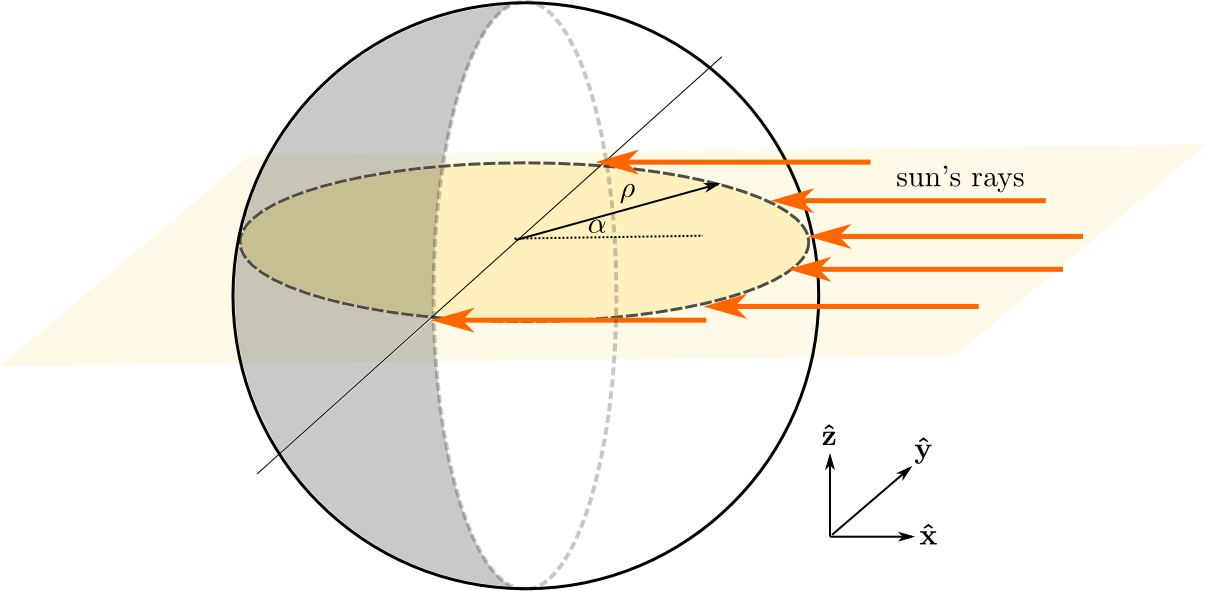
\includegraphics[width=150mm]{sphere_rhohat_horizontal2.png}
	\caption{An illustration of the intermediate step onto projecting the path of the sun's rays onto the cylindrical radius vector.}
	\label{fig:horiz_crosssect}
\end{figure}

\begin{figure}[!h]
	\centering
		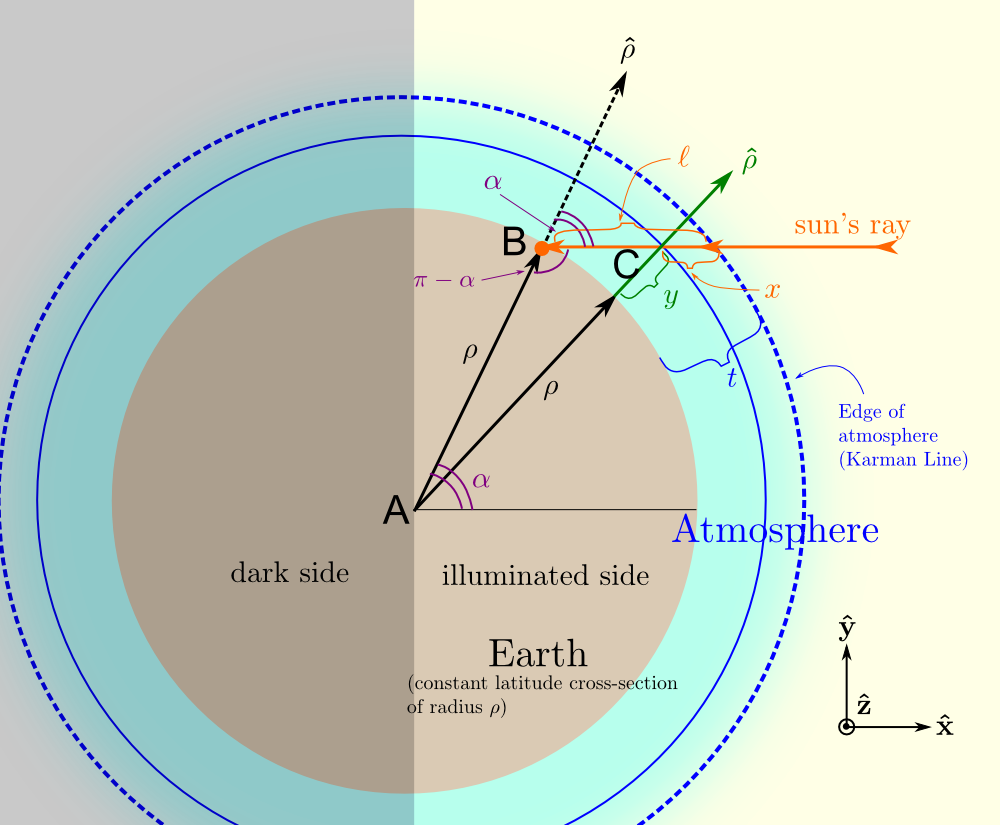
\includegraphics[width=160mm]{sphere_rhohat_fin.png}
	\caption{The geometric picture from which we will formulate most of our relevant equations in \S \ref{subsubsec:constlat}.}
	\label{fig:rho_calc}
\end{figure}

%\FloatBarrier

\vspace{10pt}
Examine Figure \ref{fig:rho_calc} carefully; from this geometric picture we will formulate most of our equations. Using the Law of Cosines on $\bigtriangleup ABC$ in that figure, we have
\begin{align} \label{eq:lawofcosines}
(\rho+y)^2 &= \rho^2 + (\ell - x)^2 - 2\rho(\ell - x)\cos(\pi - \alpha),
\end{align}

where $\ell$ is the total path length of the light beam through the atmosphere. To simplify things, we observe that
$$
\cos(\pi - \alpha) = -\cos \alpha
$$

and define
\begin{align} \label{eq:xl-def}
x_{\ell} \equiv \ell - x.
\end{align}

Substituting these into \eqref{eq:lawofcosines}, and after some algebra and rearrangements, we get
\begin{align}
x_{\ell}^2 + (2\rho \cos \alpha) x_{\ell} + \rho^2 - (\rho+y)^2 = 0.
\end{align}

Note that this is quadratic in $x_{\ell}$. Using the quadratic equation, we find that
$$
x_{\ell} = \frac{-2\rho\cos\alpha \pm \sqrt{4\rho^2 \cos^2 \alpha - 4(\rho^2 - (\rho+y)^2)}}{2}.
$$

Since $x_{\ell}$ is strictly positive, we take the positive root. After some algebra, we get
\begin{align}\label{eq:xltoy}
\frac{x_{\ell}}{\rho} = -\cos \alpha + \sqrt{\cos^2\alpha - 1 + \left(\frac{\rho+y}{\rho}\right)^2} = -\cos \alpha + \sqrt{\left(1 + \frac{y}{\rho}\right)^2 - \sin^2 \alpha},
\end{align}

where we have used the Pythagorean identity $1-\cos^2 \alpha = \sin^2 \alpha$ in the last equality.

\subsubsection{Projecting onto Earth's Radial Vector}
\label{subsubsec:radial_vec}
Now that we have $y$, we can project that onto the radial/normal vector $\mathbf{\hat{r}}$ to find $z$, the height above the ground. In a spherically symmetric planet, "`up"' is directly normal to the surface. Consider Figure \ref{fig:r_calc}.

\begin{figure}[!h]
	\centering
		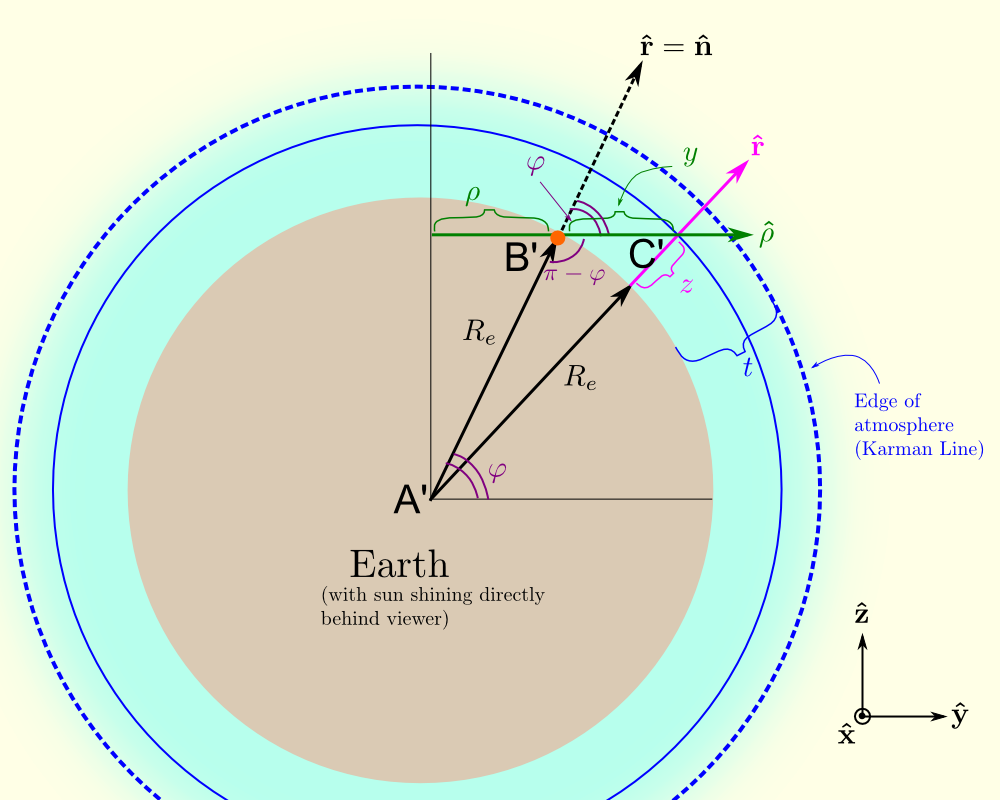
\includegraphics[width=160mm]{sphere_rhat2.png}
	\caption{The geometric picture from which we will formulate most of our relevant equations in \S \ref{subsubsec:radial_vec}. Compare to Figure \ref{fig:rho_calc}.}
	\label{fig:r_calc}
\end{figure}

\vspace{10pt}
Compare this now to Figure \ref{fig:rho_calc}. Note the similarities, and differences. (One of them is that we're looking at the Earth now from the same direction as the sun's rays, instead of perpendicular to the sun's rays, onto a particular cross section.)

\vspace{10pt} Upon further inspection of Figure \ref{fig:r_calc}, we see that the governing Law of Cosines equation (Eqn \eqref{eq:lawofcosines}) applies here as well for $\bigtriangleup A'B'C'$. This exposes the symmetry between the latitudinal dependence and the temporal dependence of the path length of the Sun's rays. Hence, we can reuse our result for $y$, Eqn \eqref{eq:xltoy}, and just switch out the variables:
\begin{gather*}
y \rightarrow z \\
x_{\ell} \rightarrow y \\
r \rightarrow R_e \\
\alpha \rightarrow \varphi.
\end{gather*}

From this we get
\begin{align}\label{eq:ytoz}
\frac{y}{R_e} = -\cos \varphi + \sqrt{\left(1 + \frac{z}{R_e}\right)^2 - \sin^2 \varphi}.
\end{align}

We can then expand the binomial term in the square root, and observing that $z \ll R_e$ through the ranges we are interested in, such that $z^2 / R_e^2 \approx 0$,
\begin{align}\label{eq:ytoz2}
\frac{y}{R_e} = -\cos \varphi + \sqrt{\left(1 + \frac{2z}{R_e} + \frac{z^2}{R_e^2}\right) - \sin^2 \varphi} \simeq -\cos \varphi + \sqrt{\cos^2\varphi + \frac{2z}{R_e}},
\end{align}

where we have again used the Pythagorean identity.

\vspace{10pt} On a related note, we can also relate the cross-section radius to Earth's radius. Recall from spherical coordinates that the cylindrical radius $\rho$ is related to the radius of the sphere $R_s$ by
$$
\rho = R_s \sin \theta,
$$

where $\theta$ is the polar angle in spherical coordinates, and $R_s = R_e =$ the spherical Earth's radius. However, observe from Figure \ref{fig:r_calc} that the latitude $\varphi = \pi/2 - \theta$. Hence,
\begin{align} \label{eq:rtophi}
\rho = R_e \sin (\pi/2 - \varphi) = R_e \cos \varphi.
\end{align}

With everything set up, we can go back to equation \eqref{eq:xltoy} and eliminate the variables $y$ and $\rho$. From \eqref{eq:rtophi} and \eqref{eq:ytoz},
\begin{align}
1+\frac{y}{\rho} &= 1 + \frac{y}{R_e}\frac{1}{\cos \varphi} \nonumber \\
&= 1 + \frac{1}{\cos \varphi} \left( -\cos \varphi + \sqrt{\cos^2\varphi + \frac{2z}{R_e}}\right) = \sqrt{1 + \frac{2z}{R_e} \sec^2 \varphi}.
\end{align}

Inserting this expression for $1+y/\rho$ into \eqref{eq:xltoy} yields
\begin{align*}
\frac{x_{\ell}}{R_e \cos \varphi} &= -\cos \alpha + \sqrt{1 + \frac{2z}{R_e} \sec^2 \varphi - \sin^2 \alpha}.
\end{align*}

This then simplifies to
\begin{align} \label{xltoz_ALL}
\frac{x_{\ell}}{R_e} &= -\cos \alpha \cos \varphi + \sqrt{\frac{2z}{R_e} + \cos^2\alpha \cos^2\varphi}.
\end{align}

(Again, note the symmetry betwen $\alpha$ and $\varphi$.)

\subsection{Completing the Integration}
Now we are ready to take derivatives to convert our $x$-coordinate in \eqref{eq:ln_i-i0} to the $z$-coordinate in \eqref{eq:ndensity}. From \eqref{eq:xl-def}
$$
\frac{dx}{dz} = -\frac{dx_{\ell}}{dz}.
$$
But from \eqref{xltoz_ALL},
\begin{align}
\frac{dx_{\ell}}{dz} = \left(\frac{2z}{R_e} + \cos^2\alpha \cos^2\varphi \right)^{-1/2}.
\end{align}

Putting the two together,
\begin{align}
dx = -\left(\frac{2z}{R_e} + \cos^2\alpha \cos^2\varphi \right)^{-1/2} dz.
\end{align}

Combining this with our isothermal atmosphere assumption \eqref{eq:ndensity}, our integral in \eqref{eq:ln_i-i0} becomes (for a light beam that travels all the way to the ground)
\begin{align} \label{eq:optthickness}
-\tau \equiv \ln \left(\frac{I}{I_0}\right) = \int_{t}^0 \sigma n_0 e^{-z/H} \left(\frac{2z}{R_e} + \cos^2\alpha \cos^2\varphi \right)^{-1/2} dz,
\end{align}

where $t$ is the thickness of the atmosphere, and $\tau$ is the \textit{optical thickness} of the atmosphere. And we've pretty much done what we've set out to do, as now this integral is much easier to compute. Define
$$
\zeta \equiv \frac{R_e}{2H}\left(\frac{2z}{R_e} + \beta^2 \right) = \frac{z}{H} + \frac{R_e\beta^2}{2H}
$$

where
\begin{align} \label{eq:beta-def}
\beta^2 \equiv \cos^2 \alpha \cos^2 \varphi.
\end{align}

However, it turns out that since the number density of molecules outside of $t$ is negligible anyway, we can extend our that integration limit to infinity to simplify our math. Using a change of variable to $\zeta$, our integral in \eqref{eq:optthickness} becomes

\begin{align}
\tau &= \lim_{t \to +\infty} \int_{R_e \beta^2 / 2H}^{t} \sigma n_0 \exp\left[-\left(\zeta - \frac{R_e \beta^2}{2H}\right)\right] \left(\frac{2H}{R_e}\zeta\right)^{-1/2} (H \: d\zeta) \nonumber \\[0.4em] \label{eq:simplestint}
&= \sigma n_0 \sqrt{\frac{R_e H}{2}}\exp\left(\frac{R_e \beta^2}{2H}\right)\int_{R_e \beta^2 / 2H}^{\infty}  \zeta^{-1/2} e^{-\zeta} \: d\zeta. 
\end{align}

Consider that
$$
\int_a^{\infty} u^{-1/2} e^{-u} \: du = \sqrt{\pi} \erfc\left(\sqrt{a}\right),
$$

where $\erfc(x)$ is the complementary error function
$$
\erfc(x) =  1- \frac{2}{\sqrt{\pi}} \int_0^x e^{-t^2} \: dt.
$$

Hence,
\begin{align}
\int_{R_e \beta/2H}^{\infty} \zeta^{-1/2} e^{-\zeta} \: d\zeta = \sqrt{\pi} \erfc\left({\sqrt{\frac{R_e \beta^2}{2H}}}\right).
\end{align}

Plugging this integral into the whole expression in \eqref{eq:simplestint}, we get

\begin{equation}
\boxed{
\begin{aligned} 
 \tau &= \sigma n_0 \sqrt{\frac{\pi R_e H}{2}} \exp\left(\frac{R_e \beta^2}{2H}\right) \erfc\left({\sqrt{\frac{R_e \beta^2}{2H}}}\right)  \\[0.4em]
&= \sigma n_0 \sqrt{\frac{\pi R_e H}{2}} \exp\left(\frac{R_e}{2H} \cos^2\alpha \cos^2\varphi \right) \erfc\left({\sqrt{\frac{R_e}{2H}}\cos\alpha \cos\varphi}\right) = -\ln \left(\frac{I}{I_0}\right). \label{eq:i-i0-exact}
\end{aligned} }
\end{equation}

\subsection{Approximations}
$\erfc(x)$ has the following asymptotic series expansion for $x \gg 1$:
$$
\erfc(x) \simeq e^{-x^2}\left(\frac{1}{\sqrt{\pi} x} + \frac{1}{2\sqrt{\pi} x^3} + \cdots \right)
$$

If $x = \sqrt{R_e / 2H}\cos\alpha \cos\varphi$, we can insert the series into \eqref{eq:i-i0-exact}:
$$
\tau \simeq \sigma n_0 \sqrt{\frac{\pi R_e H}{2}} \cancel{\exp\left(\frac{R_e}{2H} \cos^2\alpha \cos^2\varphi \right)} \cancel{\exp\left(-\frac{R_e}{2H} \cos^2\alpha \cos^2\varphi \right)} \left(\sqrt{\frac{2H}{\pi R_e\cos^2\alpha \cos^2\varphi}} + O\left(\frac{H}{R_e}\right)^{3/2} + \cdots \right).
$$

Because $H/R_e \ll 1$, we can truncate terms of order $(H/R_e)^{3/2}$ and higher, leaving us with
\begin{align}
\tau \simeq \frac{\sigma n_0 H}{\cos\alpha \cos\varphi};
\end{align}
and thus
\begin{align} \label{eq:i-i0-approx}
\boxed{ \frac{I}{I_0} \simeq \exp\left(-\frac{\sigma n_0 H}{\cos\alpha \cos\varphi}\right). }
\end{align}

\subsubsection{Remarks}
The approximation assumes large values of $x$, which implies that both $\cos\varphi$ and  $\cos\alpha$ must not be near zero. In other words, the approximation breaks down near the North and South Poles and near sunrise/sunset. Nevertheless, we can get good values not too from far these extremes. For instance, at $\varphi = \alpha = 60^{\circ}$, the error from the approximation is around $1\%$. $\varphi = 60^{\circ}$N latitude crosses the southern edge of Alaska and Scandanavia. $\alpha = 60^{\circ}$ corresponds to two hours after sunrise/two hours before sunset. Not bad considering I live in California, and 2 hours before sunset is when many people start getting off work!

\vspace{10pt} Finish with tangent plane approximation.

%\subsection{Values of Attenuation}
%Now we can actually calculate numerical values for the Sun's attenuation. We use the following cosntants:
%\begin{gather*}
%H = \text{scale height} \approx 8 \text{ km} \\
%R_e = \text{radius of Earth} \approx 6400 \text{ km} \\
%\sigma = \text{average scattering cross section of air molecule} \approx 5 \times 10^{-31} \text{ m}^2 \\
%\rho_0 = \text{density of air at sea level} \approx 1.2 \text{ kg m}^{-3} \\
%M = \text{average molar mass of air} \approx 29 \text{ g mol}^{-1} \\
%n_0 = \text{number density of air molecules at sea level}=\frac{N_A \rho_0}{M} = 2.5 \times 10^{25} \text{ m}^{-3},
%\end{gather*}
%
%where $N_A$ is Avogadro's constant, $6.022 \times 10^{23}$ mol$^{-1}$. From these, we have
%\begin{gather*}
%\sigma n_0 \sqrt{\frac{\pi R_e H}{2}} \approx 3.5 \\[0.4em]
%\frac{R_e}{2H} \approx 400 \Rightarrow \sqrt{\frac{R_e}{2H}} \approx 20.
%\end{gather*}

%%%% begin perturbation: non-spherical Earth %%%%

\subsection{More about $\alpha$; Sunrise/Sunset Times}
\label{subsec:sunsetrise}

As a final note, let us clarify the physical meaning of $\alpha$. I claim that
$$
\alpha = \Omega t + \delta = \phi,
$$

where $\Omega$ is the angular velocity of Earth's rotation, $t$ is some time in the day relative to sunrise/sunset, $\delta$ is some phase shift constant, and $\phi$ is the azimuthal angle spherical coordinate. $\delta$ will depend on how we define $t$ (and vice versa) such that $\alpha = \pm \pi/2$ at sunset/sunrise, respectively. (Refer to Fig \ref{fig:rho_calc}.)

\vspace{10pt} Where applicable, for the rest of this document and for the sake of simplicity, I'm going to let $\delta \equiv 0$ such that 
\begin{align} \label{eq:alpha_def}
\alpha \equiv \Omega t,
\end{align}

such that the sunset/sunrise (+/-) time $t_s$ will occur at (for this zero axial tilt assumption)
\begin{align}
t_s = \pm \frac{\pi}{2 \Omega}.
\end{align}

In particular, note that this definition will allow for $t < 0$; keep that in mind as we move forward in our calculations.

\numberwithin{equation}{section}
\numberwithin{figure}{section}
\section{Incorporating Axial Tilt/Obliquity}

We now begin a series of sections that will stress our basic case, remove assumptions one by one independently, and observe the effects. First, we will consider adding in an axial tilt. 

\subsection{Defining Axial Tilt; Coordinate Systems}

We shall define the axial tilt $\psi$ as the angle between the orbital plane and the equatorial plane, or equivalently the angle between the vector normal to the orbital plane and the Earth's axis of rotation. See Figure \ref{fig:axialtilt}. Currently $\psi$ for Earth is about 23.4$^{\circ}$.

\begin{figure}[!h]
	\centering
		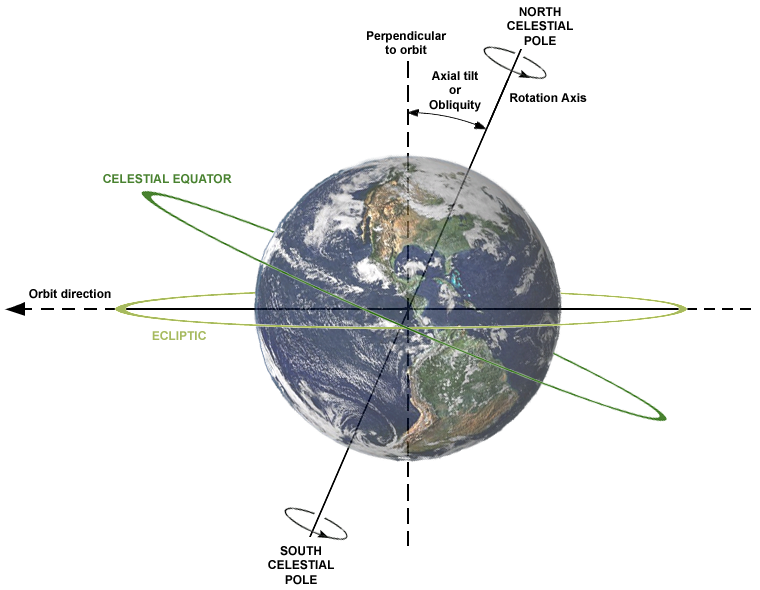
\includegraphics[width=150mm]{AxialTiltObliquity.png}
	\caption{An illustration of the definition of axial tilt. Illustration from \href{http://en.wikipedia.org/wiki/File:AxialTiltObliquity.png}{Wikipedia}.}
	\label{fig:axialtilt}
\end{figure}

\vspace{10pt}
Now, for the coordinates. The solution we seek is simple if we could rotate our simple case solution about some axis. But here's the problem. Suppose we define $\mathbf{\hat{X}}$ and $\mathbf{\hat{Y}}$ as unit vectors that span the orbital plane. We can define a rotation $\psi$ around $\mathbf{\hat{X}}$, but it wouldn't matter because at different points $+\mathbf{\hat{X}}, -\mathbf{\hat{X}}, +\mathbf{\hat{Y}}, -\mathbf{\hat{Y}}$ the direction of the sun's rays would not be the same.

\vspace{10pt}
The solution is to use \emph{Earth-relative coordinates}: coordinates that are aligned with the relative position of the Earth and Sun. Let $\mathbf{\hat{x}}$ point towards the direction of the Sun's rays at all times, in agreement with Figures \ref{fig:rho_calc} and \ref{fig:r_calc}, and $\mathbf{\hat{z}}$ point in the same direction as $\mathbf{\hat{Z}}$, that is, perpendicular to the orbital plane. Let $\mathbf{\hat{y}}$ be such that $\mathbf{\hat{x}} \times \mathbf{\hat{y}} = \mathbf{\hat{z}}$. Note that this is not necessarily tangent to the orbit as the Earth's orbit is elliptical. All this is summarized in Figure \ref{fig:axialtilt_coords}.

\begin{figure}[!h]
	\centering
		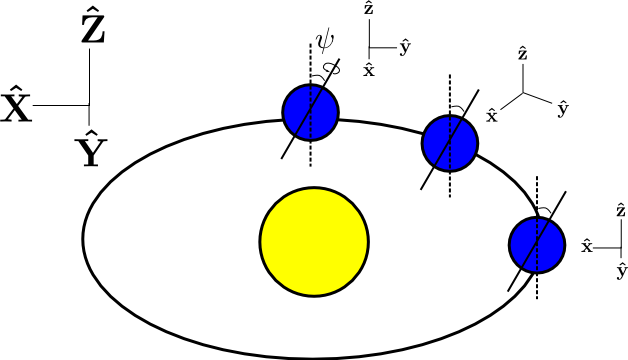
\includegraphics[width=140mm]{axialtilt_coords.png}
	\caption{Earth-relative and orbital plane relative coordinates.}
	\label{fig:axialtilt_coords}
\end{figure}

\vspace{10pt} The tradeoff now is the rotation we must apply varies with location along the orbit. Later we will develop the machinery to transform between $\left\{ \mathbf{\hat{X}}, \mathbf{\hat{Y}}, \mathbf{\hat{Z}} \right\}$ and $\left\{ \mathbf{\hat{x}}, \mathbf{\hat{y}}, \mathbf{\hat{z}} \right\}$ in general. Initially we will consider a couple of special cases before moving onto the general case.

\subsection{Notation, and preliminaries}

A quick note on notation. 

\begin{enumerate}
 \item We will use $(x, y, z)$ for coordinates along the $\mathbf{\hat{x}}, \mathbf{\hat{y}}, \mathbf{\hat{z}}$ axes (which are fixed from the Earth frame of reference).
 \item We will use $(x_0, y_0, z_0)$ for values of $(x, y, z)$ without incorporating the axial tilt.
 \item We will use $(x', y', z')$ for values of $(x, y, z)$ after incorporating the axial tilt.
\end{enumerate}

Actually the second of the above is easy to find, because we can just use our normal spherical coordinate transformation formula with the origin at the center of the earth. Without the axial tilt, the rotation of a point at latitude $\varphi$ on a spherical earth is given in column-vector form, in local Cartesian coordinates relative to the center of the Earth, as follows:
\begin{align} \label{eq:noaxialtilt}
\left[ \begin{array}{ccc}
	x_0 \\
	y_0 \\
	z_0 \\
\end{array} \right] =  \left[ \begin{array}{ccc}
	\rho \cos \Omega t \\
	\rho \sin \Omega t\\
	R_e \sin \varphi \\
\end{array} \right] =  \left[ \begin{array}{ccc}
	R_e \cos \varphi \cos \Omega t \\
	R_e \cos \varphi \sin \Omega t\\
	R_e \sin \varphi \\
\end{array} \right],
\end{align}
where $\rho \equiv R_e \cos \varphi$. (Recall our definition of $t$ was such that $t=0$ coincided with zenith during the day, see \S \ref{subsec:sunsetrise} and Figure \ref{fig:horiz_crosssect}.)

\vspace{10pt}
One more thing: recall Eqs. \ref{eq:beta-def} and \ref{eq:alpha_def}; we have as a result
\begin{align} \label{eq:x-component}
\beta = \cos \alpha \cos \varphi = \cos \Omega t \cos \varphi = \cos \Omega t \sin \theta = \frac{x}{R_e},
\end{align}
again using the typical spherical coordinate transformation formula, where $\theta$ is the usual polar angle, and $x$ being what it is implied above in point (1). Now compare Eq. \eqref{eq:x-component}, and Eqs. \eqref{eq:i-i0-exact} and \eqref{eq:i-i0-approx}.

\vspace{10pt}
\textbf{Upshot:} Really, only $x'$ matters for our calculation, because only the $x$-component stuff goes into our attenuation equations! Furthermore, we can reuse Eqs. \eqref{eq:i-i0-exact} and \eqref{eq:i-i0-approx}, just finding what $\beta$ is. This will make our subsequent computations much easier (though, for completeness, we will calculate all components initially).

\subsection{The Equinoxes}

Referring to Figure \ref{fig:axialtilt_coords}, we see that the equinox occurs when the rotation of $\psi$ occurs around $\mathbf{\hat{x}}$, (the top Earth in the figure, where the tilt does not affect the relative sunlight exposure in the two hemispheres). 
Again gleaming at the figure, it is evident that the transformation we seek corresponds to a \emph{rotation} $\mathcal{R}$ of the original motion by $\psi$ about the $x$-axis. Hence we have\footnote{The matrix corresponding to a rotation transformation, $\mathcal{R}$, can be found here: \url{http://en.wikipedia.org/wiki/Rotation_matrix}}

\begin{align}
\left[ \begin{array}{c}
	x' \\
	y' \\
	z' \\
\end{array} \right] 
&=  \mathcal{R}_x (\psi)
\left[ \begin{array}{c}
	x_0 \\
	y_0 \\
	z_0 \\
\end{array} \right] \nonumber \\[0.6em] 
&=
\left[ \begin{array}{ccc}
	1 & 0 & 0 \\
	0 & \cos \psi & - \sin \psi \\
	0 & \sin \psi & \cos \psi \\
\end{array} \right]
\left[ \begin{array}{ccc}
	R_e \cos \varphi \cos \Omega t \\
	R_e \cos \varphi \sin \Omega t\\
	R_e \sin \varphi \\
\end{array} \right] \nonumber \\[0.6em]
&=
\left[ \begin{array}{c}
	R_e \cos \varphi \cos \Omega t \\
	R_e \cos \varphi \cos \psi \sin \Omega t - R_e \sin \psi \sin \varphi \\
	R_e \cos \varphi \sin \psi \sin \Omega t + R_e \cos \psi \sin \varphi \\
\end{array} \right].
\end{align}

But as we discussed earlier, only $x'$ matters and that doesn't change! So Eqs. \eqref{eq:i-i0-exact} and \eqref{eq:i-i0-approx} for zero axial tilt also apply to the equinoxes - both the fall and spring - and for both the Northern and Southern Hemisphere. 

\subsection{The Solstices}

\subsubsection{Northern Hemisphere Winter}

In Figure \ref{fig:axialtilt_coords}, the Earth on the right-hand side corresponds to the northern hemisphere winter, as the northern hemisphere is further from the Sun. Again from the figure, we see the proper rotation to use is one about the $-y$ axis.

\begin{align}
\left[ \begin{array}{c}
	x' \\
	y' \\
	z' \\
\end{array} \right] 
&=  \mathcal{R}_{-y} (\psi)
\left[ \begin{array}{c}
	x_0 \\
	y_0 \\
	z_0 \\
\end{array} \right] 
= \mathcal{R}_{y} (-\psi)
\left[ \begin{array}{c}
	x_0 \\
	y_0 \\
	z_0 \\
\end{array} \right] \nonumber \\[0.6em] 
&=
\left[ \begin{array}{ccc}
	\cos \psi  & 0 & -\sin \psi \\
	0 & 1 & 0 \\
	\sin \psi & 0 & \cos \psi \\
\end{array} \right]
\left[ \begin{array}{ccc}
	R_e \cos \varphi \cos \Omega t \\
	R_e \cos \varphi \sin \Omega t\\
	R_e \sin \varphi \\
\end{array} \right] \nonumber \\[0.6em]
&=
\left[ \begin{array}{c}
	R_e \cos \varphi \cos \Omega t \cos \psi - R_e \sin \varphi \sin \psi \\
	R_e \cos \varphi \sin \Omega t \\
	R_e \cos \varphi \sin \Omega t \sin \psi + R_e \sin \varphi \cos \psi \\
\end{array} \right].
\end{align}

Hence,
\begin{align}
\beta = \frac{x'}{R_e} = \cos \varphi \cos \Omega t \cos \psi - \sin \varphi \sin \psi,
\end{align}

and the approximate formula for $I/I_0$ is

\begin{align} \label{eq:i-i0-approx-winter}
\boxed{ \frac{I}{I_0} \simeq \exp\left(-\frac{\sigma n_0 H}{\cos \varphi \cos \Omega t \cos \psi - \sin \varphi \sin \psi}\right). }
\end{align}

\subsubsection{Northern Hemisphere Summer}
This is really similar to the winter case, except you rotate about the positive $y$-axis instead of the negative. In other words, use $\mathcal{R}_y (\psi)$ instead of $\mathcal{R}_y(-\psi)$. This amounts to swapping the signs on the sin,
\begin{align}
\left[ \begin{array}{c}
	x' \\
	y' \\
	z' \\
\end{array} \right] =
\left[ \begin{array}{c}
	R_e \cos \varphi \cos \Omega t \cos \psi + R_e \sin \varphi \sin \psi \\
	R_e \cos \varphi \sin \Omega t \\
	-R_e \cos \varphi \sin \Omega t \sin \psi + R_e \sin \varphi \cos \psi \\
\end{array} \right],
\end{align}

so that
\begin{align}
\beta = \frac{x'}{R_e} = \cos \varphi \cos \Omega t \cos \psi + \sin \varphi \sin \psi,
\end{align}
\begin{align}
\boxed{ \frac{I}{I_0} \simeq \exp\left(-\frac{\sigma n_0 H}{\cos \varphi \cos \Omega t \cos \psi + \sin \varphi \sin \psi}\right). }
\end{align}

\subsubsection{Sanity check}
Before we move on, let's do a quick sanity check to make sure our calculations. First, if $\psi$ was zero:
Finish.

\subsection{General Case}

Given that we applied a rotation about the local $\mathbf{\hat{x}}$ and $\mathbf{\hat{y}}$ axes for the equinox and solstice calculation, respectively, it would make sense to apply a rotation about a general vector $\mathbf{u} = (u_x, u_y, 0)$ on the $xy$-plane for the general calculation of incorporating obliquity.

\vspace{10pt}
The generalized rotation matrix is given by\footnote{Adapted from link in previous footnote.}
\begin{align}
R_{\mathbf{u}}(\psi)
\left[ \begin{array}{ccc}
	\cos \psi + u_x^2 (1-\cos \psi) & u_x u_y (1-\cos \psi) & u_y \sin \psi \\
	u_x u_y (1-\cos \psi) & cos \psi + u_y^2 (1-\cos \psi) & -u_x \sin \psi \\
	-u_y \sin \psi &  u_x \sin \psi & \cos \psi\\
\end{array} \right]
\end{align}.

Again using only the $x$-component, we get
\begin{align} \label{eq:generalcase_start}
\beta = \frac{x'}{R_e} &= (\cos \psi + u_x^2 (1-\cos \psi))\cos \varphi \cos \Omega t + u_x u_y (1-\cos \psi)\cos \varphi \sin \Omega t + u_y \sin \psi \sin \varphi.
\end{align}

\subsubsection{The True Anomaly}

The crux of the problem now becomes how we can figure out $u_x$ and $u_y$. To figure this out, we introduce a new parameter, the \emph{true anomaly}.

\vspace{10pt}
Consider the two-body problem posed by Kepler, with a massive sun and a small planet orbiting the sun being held by inverse-square force (namely, gravity). The solution to this problem, as Kepler deduced, was an elliptical orbit with the sun at a focus of the ellipse. This is mainly correct; the other planets perturb this orbit but we'll neglect that perturbation for now.

\vspace{10pt}
Some terminology: the point in the orbit closest to the sun is called $\emph{perihelion}$. The point furthest is the $\emph{aphelion}$. The angular position of the planet relative to the perihelion is the true anomaly. This is summarized in the following figure:

\vspace{10pt}FIGURE.

\vspace{10pt}
As it turns out, the slight difference between the perihelion and aphelion distances from the sun do not matter much in terms of the radiation flux. So we proceed with the true anomaly. At some point in the orbit, at some true anomaly, the axial tilt will be a rotation about $\mathbf{\hat{x}}$. At some other point it will be $\mathbf{\hat{y}}$, and so on. So our problem of finding $u_x$ and $u_y$ is reduced to finding those as a function of the true anomaly, which we'll call $\nu$. 

\vspace{10pt}
The point in the orbit where the axial tilt is a rotation about $\mathbf{\hat{x}}$ is a particularly nice reference point, so let's call that point $\nu_0$. Let's say, for sake of argument, $\nu_0 = 0$. From Figure (number), we can easily see that $u_x = \cos \nu$, and $u_y = \sin \nu$.

\vspace{10pt}FIGURE.

\vspace{10pt}
\emph{Conclusion}: without loss of generality, for any $\nu_0$, 
\begin{align}
u_x &= \cos (\nu - \nu_0) = \cos \bar{\nu}, \\ 
u_y &= \sin (\nu - \nu_0) = \sin \bar{\nu},
\end{align}
where we have defined $\bar{\nu} \equiv \nu - \nu_0$.

\vspace{10pt}
Inserting our result above into Eq. \eqref{eq:generalcase_start}, and after some trigonometric manipulation, we get
\begin{align}
\beta = (\cos \psi \sin^2\bar{\nu} + \cos^2\bar{\nu})\cos \varphi \cos \Omega t + \sin 2\bar{\nu} \sin^2\frac{\psi}{2} \cos \varphi \sin \Omega t + \sin \bar{\nu} \sin \psi \sin \varphi.
\end{align}


\numberwithin{equation}{section}
\numberwithin{figure}{section}
\section{Non-Spherical Perturbation}

% add what the series are.

Due to the effects of Earth's rotation, the Earth is not a perfect sphere. Its shape is best approximated by an \emph{oblate spheroid}, essentially a sphere that is flattened at the poles relative to the equator. The axial symmetry is retained.

\vspace{10pt} Recall our logic worked out in the ideal case:

$$
\boxed{x_{\ell} \leftarrow y \leftarrow z} \Rightarrow \frac{dx_{\ell}}{dz} \Rightarrow \frac{dx}{dz} \Rightarrow d\tau \Rightarrow \text{Integrate.}
$$

Because of the axial symmetry, the left-most arrow in the box -- projecting the path of a light ray onto the cylindrical radius vector -- remains the same. (See \S \ref{subsubsec:constlat}.) But subsequently projecting that projection onto the normal vector to the oblate spheroid -- which will differ from the radial vector -- takes some more work.

\subsection{Variation of Oblate Spheroid Radius}
\label{subsec:varrad}

Let the larger equatorial radius be $a$, polar radius be $b$. The eccentricity $e$, a measure of deviation from perfect sphericity, is defined by
\begin{align} \label{eq:eccentricity}
e^2 = 1 - \frac{b^2}{a^2}.
\end{align}

The projection of an oblate spheroid to a plane perpendicular to the equatorial axis is an ellipse. The equation of such an ellipse in plane-polar coordinates (r, $\theta$) is,
\begin{align} \label{eq:ellipseb}
r(\theta) = \frac{ab}{\sqrt{b^2 \cos^2 \theta + a^2 \sin^2 \theta}}.
\end{align}

Substituting the eccentricity in for $b$, that is, from \ref{eq:eccentricity} and \ref{eq:ellipseb}, we get
\begin{align} \label{eq:ellipsee}
r(\theta) = \frac{a \sqrt{1-e^2}}{\sqrt{1 - e^2 \cos^2 \theta}}.
\end{align}

Since the Earth is only slightly aspherical -- $b$ is only smaller than $a$ by around 20 miles -- $e \ll 1$. Thus we can Taylor expand the square-root factors:
\begin{align*}
r(\theta) &\simeq a \left(1-\frac{e^2}{2} + \cdots \right) \left(1+\frac{e^2 \cos^2 \theta}{2} + \cdots \right) \\[0.5em]
&= a\left(1 - \frac{e^2}{2}(1 - \cos^2 \theta) + O(e^4) + \cdots \right).
\end{align*}

Neglecting terms of order higher than $e^2$ and using the Pythogorean identity, we get
\begin{align} \label{eq:ellipsee_approx}
r(\theta) \simeq a \left(1 - \frac{e^2}{2} \sin^2 \theta\right).
\end{align}

\subsubsection{Remarks on $\theta$}

Assuming the center of the Earth-body rests at the origin, it is easily shown that the plane-polar coordinate $\theta$ in the 2-space of the ellipse is related to the spherical polar angle $\tilde{\theta}$ in the 3-space containing the unprojected oblate spherioid by $\theta = \pi / 2 -\tilde{\theta} $. Hence, 
$$
\theta = \varphi_c,
$$

where $\varphi_c$ is the \emph{geocentric} latitude as before in \S \ref{sec:basic}. This angle is formed by the \emph{radial} vector at a point to the equatorial plane. However, the latitude that the field of geodesy uses is the \emph{geodetic} latitude, the angle formed by the \emph{normal} vector at a point to the equatorial plane. We will refer the geodetic latitude in subsequent calculations with symbol $\varphi_{d}$. Additionally, we will use $\varphi_c$ in favor of $\theta$.

\begin{figure}[!h]
	\centering
		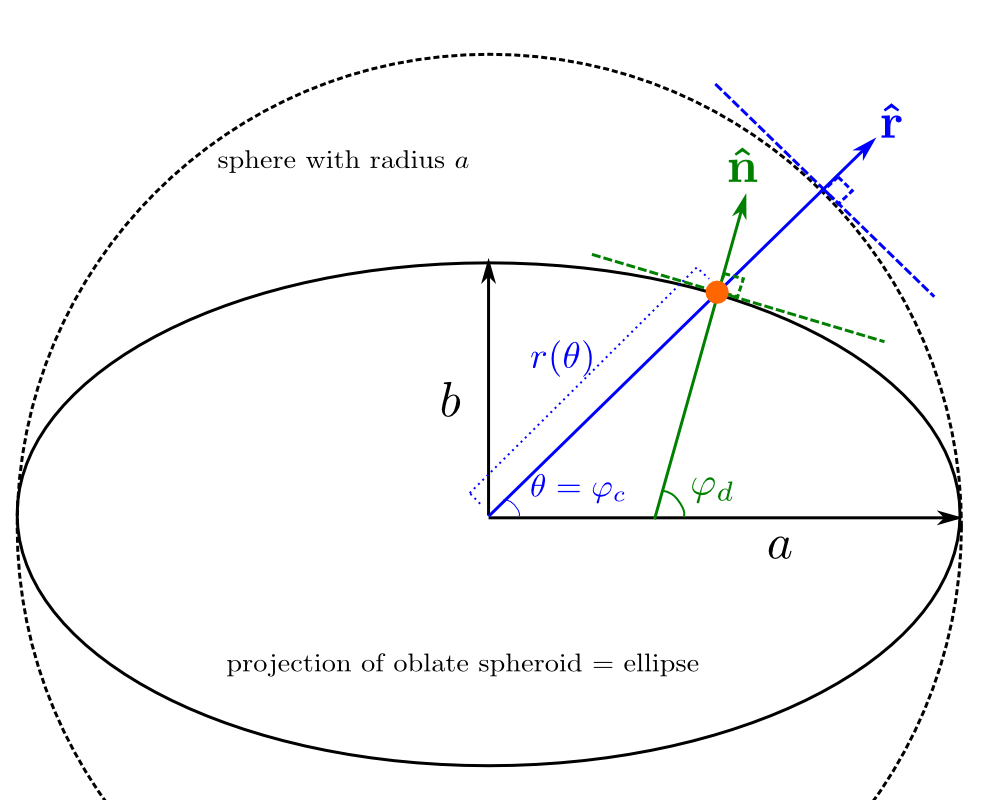
\includegraphics[width=130mm]{spheroid_1b.png}
	\caption{Relationship between geocentric and geodetic latitudes.}
	\label{fig:geodeticlat}
\end{figure}
%\FloatBarrier

\subsection{Geometric Governing Equations}

As before, we begin the meat of our calculations with an illustration of the geometry of the problem in Figure \ref{fig:spheroid_geom}.

\begin{figure}[!h]
	\centering
		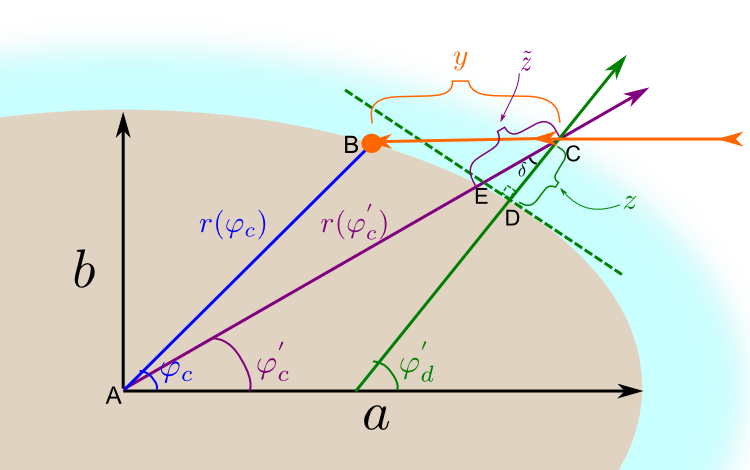
\includegraphics[width=130mm]{spheroid_2.png}
	\caption{Geometric setup for the calculation of oblate spheroid perturbation, and definitions of relevant angles/lengths.}
	\label{fig:spheroid_geom}
\end{figure}
%\FloatBarrier
\vspace{10pt}
From Figure \ref{fig:spheroid_geom}, we can obtain the following equations:

\begin{enumerate}

\item Using the Law of Cosines on $\bigtriangleup ABC$ (a familiar step):
\begin{align} \label{eq:lawcosines_spheroid}
(r(\varphi_c^{'}) + \tilde{z})^2 = y^2 + r(\varphi_c)^2 - 2y r(\varphi_c) \cos (\pi - \varphi_c).
\end{align}
Compare Eqn \eqref{eq:lawcosines_spheroid} to Eqn \eqref{eq:lawofcosines}.

\item Using the Law of Sines on $\bigtriangleup ABC$:
\begin{align} \label{eq:lawsines_spheroid}
\frac{\sin (\varphi_c - \varphi_c^{'})}{y} = \frac{\sin \varphi_c^{'}}{r(\varphi_c)}
\end{align}

\item From $\bigtriangleup CDE$:
\begin{align} \label{eq:ztilde-z}
z \simeq \tilde{z} \cos(\varphi_d^{'} - \varphi_c^{'}).
\end{align}

\item The relationship between geodetic latitude $\varphi_d^{'}$ and geocentric latitude $\varphi_c^{'}$ for a given eccentricity $e$ (we will simply quote this formula without proof):
\begin{align} \label{eq:geodetic-geocentric}
\frac{\tan \varphi_d^{'}}{\tan \varphi_c^{'}} = 1 - e^2.
\end{align}

\end{enumerate}

Recall we are trying to find a relationship between $z$ and $y$ (see the beginning of this section). There are three additional unknowns: $\varphi_c^{'}$, $\varphi_d^{'}$, and $\tilde{z}$. Four equations. So we're good. Solving these four simultaneous equations -- that's another story. We'll need to make some serious approximations.

\subsubsection{Combining Eqs. \eqref{eq:ztilde-z} and \eqref{eq:geodetic-geocentric}}

If $\varphi_d^{'}$ is close to $\varphi_c^{'}$, we can Taylor expand Eqn \eqref{eq:ztilde-z} about $\varphi_d^{'} - \varphi_c^{'}$:
$$
z \simeq \tilde{z} \left( 1-\frac{(\varphi_d^{'} - \varphi_c^{'})^2}{2} + \cdots \right).
$$

From Eqn \eqref{eq:geodetic-geocentric}
$$
\tan \varphi_d^{'} - \tan \varphi_c^{'} = - e^2 \tan \varphi_c^{'},
$$

and using the identity
$$
\tan \varphi_d^{'} - \tan \varphi_c^{'} = \frac{\sin (\varphi_d^{'}-\varphi_c^{'})}{\cos \varphi_d^{'} \cos\varphi_c^{'}},
$$

we obtain
\begin{align}
\varphi_d^{'}-\varphi_c^{'} \simeq \sin (\varphi_d^{'}-\varphi_c^{'}) = - e^2 \sin \varphi_c^{'} \cos \varphi_d^{'}.
\end{align}

Note that sin and cos are less than or equal to one for all angles, hence
$$
\varphi_d^{'}-\varphi_c^{'} \sim e^2
$$

and so
$$
z \simeq \tilde{z} (1 + O(e^4) + \cdots).
$$

\textbf{The upshot}: since $e \ll 1$, to a reasonable approximation,
\begin{align}
z \simeq \tilde{z}.
\end{align}

And so we can replace $\tilde{z}$ with $z$ everywhere.

\subsubsection{Perturbation of angle and radius}

For sake of convenience, let's define
$$
\Delta \varphi_c \equiv \varphi_c - \varphi_c^{'}.
$$

With this substitution, Eqn \eqref{eq:lawsines_spheroid} becomes
$$
\frac{r(\varphi_c)}{y} = \frac{\sin (\varphi_c - \Delta \varphi_c)}{\sin \Delta \varphi_c}.
$$ 

Then using an angle sum/difference formula, we get
$$
\frac{r(\varphi_c)}{y} = \frac{\sin \varphi_c \cos \Delta \varphi_c - \cos \varphi_c \sin \Delta \varphi_c}{\sin \Delta \varphi_c} = \frac{\sin \varphi_c}{\tan \Delta \varphi_c} - \cos \varphi_c.
$$

Hence,
\begin{align}
\tan \Delta \varphi_c = \frac{\sin \varphi_c }{r(\varphi_c) / y + \cos \varphi_c}
\end{align}

But, we note that (1) $\Delta \varphi_c \ll 1$, and (2) $\cos \varphi_c \sim 1 \ll r(\varphi_c) / y$. This yields a much more illuminating and useful result,
\begin{align} \label{eq:dphi}
\Delta \varphi_c \simeq \frac{y }{r(\varphi_c)} \sin \varphi_c.
\end{align}

Now for the radius difference between the angles. Recall the work in \S\ref{subsec:varrad} and Eqn \eqref{eq:ellipsee_approx}.
\begin{align*}
r(\varphi_c^{'}) = r(\varphi_c - \Delta \varphi_c) &= a \left(1-\frac{e^2}{2} \sin^2 (\varphi_c - \Delta \varphi_c)\right) \\[0.4em]
&= a \left(1 - \frac{e^2}{2} (\sin \varphi_c \cos \Delta \varphi_c - \cos \varphi_c \sin \Delta \varphi_c)^2\right),
\end{align*}

where we have used another angle sum/difference formula in the final equality. We can multiple the square term out and Taylor expand in powers of $\Delta \varphi_c$:
\begin{align*}
\frac{r(\varphi_c^{'})}{a} &= 1 - \frac{e^2}{2}(\sin^2 \varphi_c \cos^2 \Delta \varphi_c + \cos^2 \varphi_c \sin^2 \Delta \varphi_c - 2\sin \varphi_c \cos \Delta \varphi_c \cos \varphi_c \sin \Delta \varphi_c) \\[0.4em]
&\simeq 1 - \frac{e^2}{2}\left(\sin^2 \varphi_c (1 - \Delta \varphi_c^2 +\cdots) + \cos^2 \varphi_c (\Delta \varphi_c^2 +\cdots) - 2\sin \varphi_c \cos \varphi_c \left(1 - \frac{\Delta \varphi_c^2}{2} +\cdots \right)  (\Delta \varphi_c +\cdots) \right).
\end{align*}

Since all the terms in the parenthesis are multiplied by $e^2$, it wouldn't make sense to take any terms higher than first order, or $O(\Delta \varphi_c^2)$ or higher, for small $\Delta \varphi_c$. Thus:
\begin{align}
\frac{r(\varphi_c^{'})}{a} &\simeq 1 - \frac{e^2}{2}(\sin^2 \varphi_c - 2\sin\varphi_c \cos\varphi_c \Delta\varphi_c + O(\Delta\varphi_c^2) +\cdots) \nonumber \\[0.4em]
&\simeq \frac{r(\varphi_c)}{a} + e^2 \sin^2\varphi_c \cos\varphi_c  \frac{y}{r(\varphi_c)},
\end{align}

where we have substituted our results in \eqref{eq:dphi} for $\Delta\varphi_c$. Not surpisingly, we now define the small length $\epsilon$
\begin{align}
\frac{\epsilon}{a} \equiv e^2 \sin^2\varphi_c \cos\varphi_c
\end{align}

and hence
\begin{align} \label{eq:rpert}
r(\varphi_c^{'}) = r(\varphi_c) + \epsilon \frac{y}{r(\varphi_c)}.
\end{align}

The omission of the $y/r$ factor in the definition of the $\epsilon$ is intentional; we will see later why. Also note that the second term in \eqref{eq:rpert} is a function of $y$, $r$, and $\varphi_c$, this will present a significant challenge as we move forward.

\subsubsection{$y$ as a function of $z$}

Remember our original goal, to find a relation between the length of the projection of the light beam path onto the cylindrical radius ($y$), and the length of the projection of the light beam path onto the normal vector ($z$). Using Eqn \eqref{eq:lawcosines_spheroid} and the result in \eqref{eq:ztilde-z}, we can do this. Rewritten, Eqn \eqref{eq:lawcosines_spheroid} looks like this:
$$
y^2 + 2y r(\varphi_c) \cos \varphi_c + r(\varphi_c)^2 - (r(\varphi_c^{'}) + z)^2 = 0.
$$

Solving the quadratic equation for $y$ yields
\begin{align}
y &= -r(\varphi_c)\cos\varphi_c + \sqrt{r(\varphi_c)^2 \cos^2\varphi_c - r(\varphi_c)^2 + (r(\varphi_c^{'}) + z)^2} \nonumber \\[0.4em] \label{eq:initeqny}
&= -r\cos\varphi_c + \sqrt{r^2 \cos^2\varphi_c - r^2 + (r + \epsilon y/r + z)^2},
\end{align}

where we have substituted our result in \eqref{eq:rpert}. Expanding the trinomial term in the parenthesis in Eqn \eqref{eq:initeqny}:
\begin{align*}
\left(r + \frac{\epsilon y}{r} + z\right)^2 &= r^2 + \cancel{\left(\frac{\epsilon y}{r}\right)^2} + z^2 + \cancel{2\frac{\epsilon yz}{r}} + 2\epsilon y + 2rz \\[0.4em]
&\simeq r^2 + z^2 + 2\epsilon y + 2rz.
\end{align*}

Here, I have decided to omit terms of third-order or greater in small lengths relative to $r$: that is, $y$, $z$, and $\epsilon$. We substitute this in \eqref{eq:initeqny}:
$$
y = -r\cos\varphi_c + \sqrt{r^2 \cos^2\varphi + z^2 + 2\epsilon y + 2rz}.
$$

Hence,
\begin{align} \label{eq:yimplicit}
\frac{y}{r\cos\varphi_c} = \frac{y}{\rho(\varphi_c)} = -1 + \sqrt{1 + \frac{z^2 + 2\epsilon y}{\rho^2} + \frac{2z}{r} \sec^2 \varphi_c},
\end{align}

where if you recall $\rho$, the cylindrical radius, is defined as
$$
\rho = r\cos\varphi_c = r\sin\theta.
$$

Now remember my remark after \eqref{eq:rpert}? The extra $y$ there makes this equation a little more difficult to solve (notice the $y$ in the sqrt and on the LHS of \eqref{eq:yimplicit}). However, it can be done in a not-too-difficult manner. With a little algebra, we see that
$$
\left(1 + \frac{y}{\rho}\right)^2 = 1 + \frac{z^2}{\rho^2} + \frac{2\epsilon}{\rho}\frac{y}{\rho} + \frac{2z}{r}\sec^2 \varphi_c.
$$

Grouping powers of $y/\rho$,


\end{document}
